\documentclass[final]{beamer} % beamer 3.10: do NOT use option hyperref={pdfpagelabels=false} !
\mode<presentation> {  %% check http://www-i6.informatik.rwth-aachen.de/~dreuw/latexbeamerposter.php for examples
  \usetheme{Berlin}    %% you should define your own theme e.g. for big headlines using your own logos
}
%height=121.92
%\usepackage[english]{babel}
\usepackage{amsmath,amsthm, amssymb, latexsym}
\usepackage[size=custom,width=182.88,height=128.92,scale=2]{beamerposter}
\usepackage{array}

\setlength{\voffset}{1in}
\setlength{\topmargin}{0in}
\setlength{\footskip}{0in}
\setlength{\headheight}{0in}
\setlength{\headsep}{0in}


\setlength{\hoffset}{0in}
\setlength{\oddsidemargin}{1.5in}
\setlength{\textwidth}{67.5in}
\parindent 0in

%\setlength{\oddsidemargin}{2.5in}
%\setlength{\topmargin}{2.5in}
%\setlength{\textwidth}{67in}
%\setlength{\textheight}{43in}

% e.g. for custom size poster
\title{Generating Safe Trajectories in Stochastic Dynamic Environments by
    Leveraging Information about Obstacle Motion}
    \author{Alex Wallar | \emph{Supervisor}: Michael Weir}
\institute{School of Computer Science, University of St Andrews}
%\date{Jul. 27th, 2011}

%\input{pstyle}


\newcommand{\Acronym}[1]{\ensuremath{{{\texttt{#1}}}}}
\newcommand{\Symbol}[1]{\ensuremath{\mathcal{#1}}}
\newcommand{\Function}[1]{\ensuremath{{\textsc{#1}}}}
\newcommand{\Constant}[1]{\ensuremath{{\texttt{#1}}}}
\newcommand{\Var}[1]{\ensuremath{{{\mathrm{#1}}}}}
\newcommand{\False}{\Constant{false}}
\newcommand{\True}{\Constant{true}}
\newcommand{\Null}{\Constant{null}}
\newcommand{\R}{\ensuremath{\mathbb{R}}}
\newcommand{\AlgoFont}[1]{\footnotesize{#1}}
\newcommand{\RefFont}[1]{\tiny{#1}}


\definecolor{boxrgb}{rgb}{0.7,0.9,0.7}
\setbeamercolor{mybox1}{fg=black,bg=boxrgb}
\setbeamercolor{mybox2}{fg=red,bg=boxrgb}

\definecolor{mathrgb}{rgb}{0.0,0.0,0.74}

\definecolor{proBlockTitleFG}{rgb}{0.95,0.95,0.00}
\definecolor{proBlockTitleBG}{rgb}{0.21,0.26,0.42}
\definecolor{proBlockBodyBG}{rgb}{0.94,0.94,0.97}


\definecolor{hTitleFG}{rgb}{0.95,0.95,0.00}
\definecolor{hAuthorFG}{rgb}{1, 1, 1}
\definecolor{hInstFG}{rgb}{1, 1, 1}
\definecolor{hInfoFG}{rgb}{1, 1, 1}
\definecolor{hBG}{rgb}{0.11,0.16,0.32}

\definecolor{mytitle_bg}{rgb}{0.4,0.4,0.4}
\newcommand{\myimp}[1]{{\textcolor{mytitle_bg}{\textbf{#1}}}}
\newcommand{\myhimp}[1]{{\textcolor{red}{\textbf{#1}}}}
\newcommand{\mymath}[1]{\textcolor{mathrgb}{#1}}

\graphicspath{{../}}

\setbeamercolor{headline}{fg=red,bg=hBG}

\setbeamertemplate{headline}{
  \leavevmode

        \begin{beamercolorbox}[wd=67.5in,ht=5.8in]{headline}


\centering
%\hspace*{3.2in}
\begin{tabular}{c}
\\[-7cm]
         \textcolor{hTitleFG}{\textbf{\huge{Dodger: Generating Safe Trajectories
               in Stochastic Dynamic Environments}}}\\[2cm]
         \textcolor{hTitleFG}{\textbf{\huge{ by Leveraging Information about Obstacle Motion}}}\\[3cm]


        \textcolor{hAuthorFG}{\textbf{\huge{\insertauthor}}}\\[1.8cm]

        \textcolor{hInstFG}{\Large{\insertinstitute}}\\[1.5cm]

       % \textcolor{hInfoFG}{{\large{http://faculty.cua.edu/plaku,
        %      \texttt{plaku@cua.edu}}}}\\[0.5cm]
\end{tabular}

        \end{beamercolorbox}

  \begin{beamercolorbox}[wd=\paperwidth]{lower separation line head}
    \rule{0pt}{3pt}
  \end{beamercolorbox}
}
\setbeamertemplate{footline}{}

\setbeamertemplate{navigation symbols}{}


\newenvironment<>{problock}[1]{%
  \begin{actionenv}#2%
      \def\insertblocktitle{
\begin{beamercolorbox}[ht=1in,center]{proBlockTitleBG}
 \vbox to 1in{\vfil \centering {\Large \textbf{#1}} \vfil}%
\end{beamercolorbox}
}

      \par%
       \setbeamerfont{block body}{size=\normalsize}
       \setbeamercolor{block title}{fg=proBlockTitleFG,bg=proBlockTitleBG}
       \setbeamercolor{block body}{fg=black,bg=white}%,bg=proBlockBodyBG}
       \setbeamercolor{itemize item}{fg=orange!20!black}
       \setbeamertemplate{itemize item}[circle]
      \usebeamertemplate{block begin}\vspace*{1cm}}
    {\par\usebeamertemplate{block end}\end{actionenv}}

\begin{document}

\vspace*{-50mm}

  \begin{frame}{}
\noindent
    \begin{columns}[t]
      \begin{column}{21.6in}
        \begin{problock}{PROBLEM FORMULATION}

\begin{columns}[c]
\column{0.5\columnwidth}
\begin{itemize}
    \item Develop a dynamic obstacle representation that
        \begin{itemize}
            \item accounts for the obstacle's motion
            \item provides higher costs for paths intersecting their trajectories
        \end{itemize}
    \item Compute a motion trajectory that:
        \begin{itemize}
            \item reaches the goal region
            \item avoids collisions with static and dynamic obstacles
            \item uses imperfect information about obstacle motion to generate a
                quantitatively safe path
        \end{itemize}
\end{itemize}
\column{0.5\columnwidth}
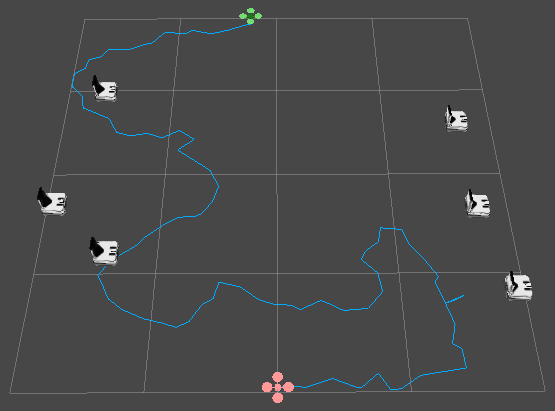
\includegraphics[width=\columnwidth]{figs/dodger_complete}
\end{columns}

\vspace*{1cm}

Utilizing information about how the obstacle will move can aid
a motion planner to generate paths that will be less likely to lead a robot
into a collision

\vspace*{3mm}

% \begin{columns}[b]
%
% \column{0.45\columnwidth}
% 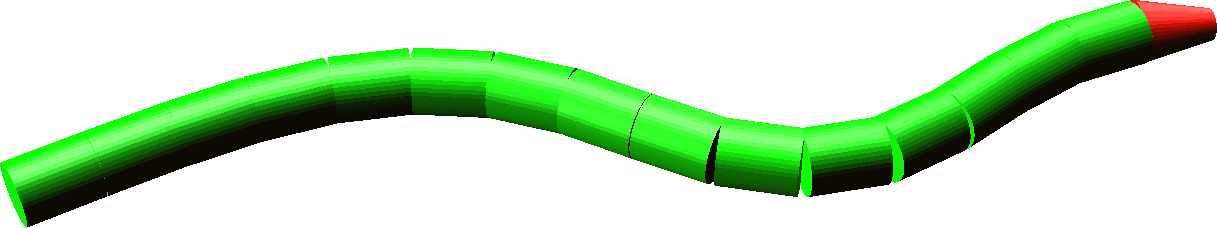
\includegraphics[width=\columnwidth]{figs/figSnake}
%
% \column{0.54\columnwidth}
% \begin{itemize}
% \item Motion dynamics can be high dimensional
% \item Often involve non-linear ODEs
% \end{itemize}
%
% \end{columns}

\vspace*{3mm}

\textcolor{red}{However, perfect information about the motion of obstacles
is almost always not readily available or easy to compute since they may veer
off their predicted trajectory}


        \end{problock}

\begin{problock}{EXPERIMENTAL RESULTS}

Average minimum distance to any obstacle compared to a potential fields
planner
\vspace*{8mm}

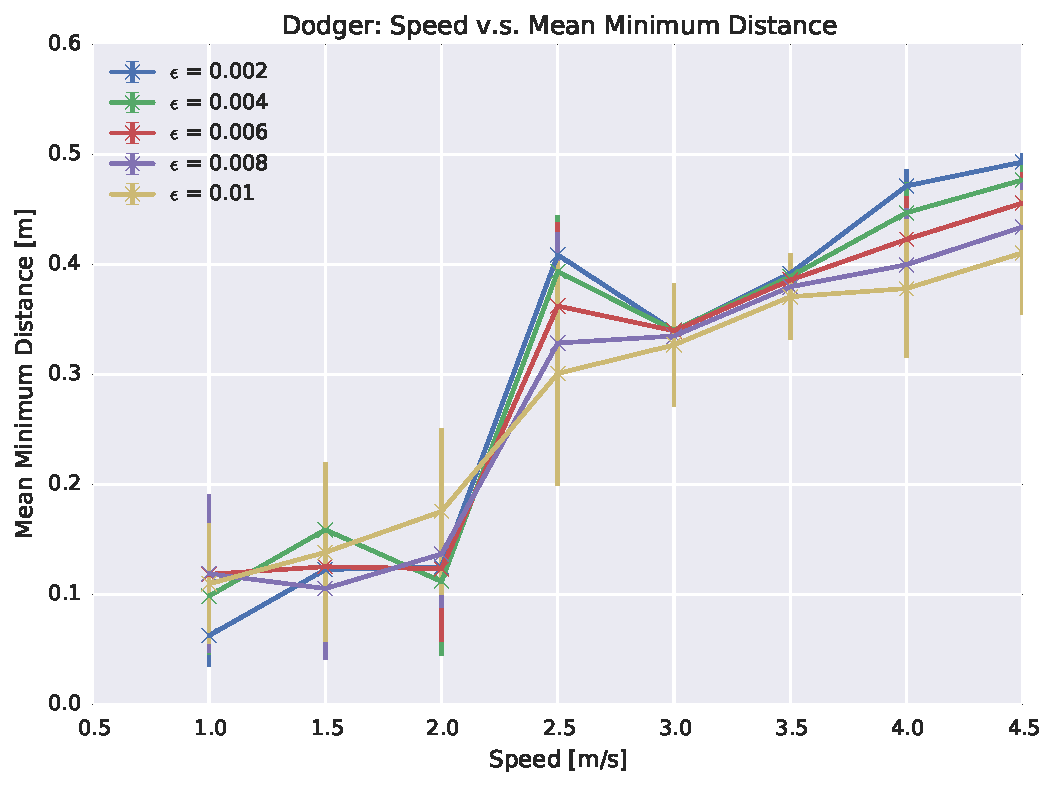
\includegraphics[width=0.49\textwidth]{figs/planner_mean_min_distance_0.pdf}
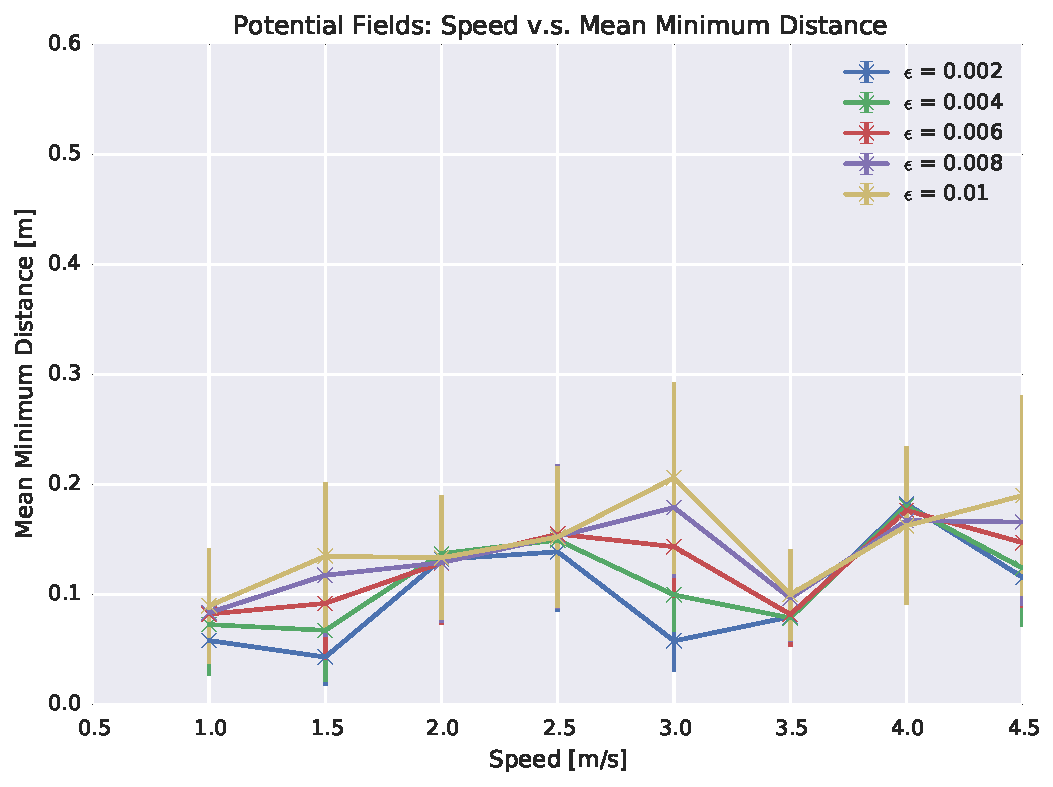
\includegraphics[width=0.49\textwidth]{figs/pf_mean_min_distance_0.pdf}

% \begin{itemize}
%     \item Each line shows a different amount of noise injected into the
%         obstacle trajectories
% \end{itemize}

\vspace*{10mm}
Maximum cost incurred by the robot along the paths generated by Dodger and
a potential fields planner. The cost is defined by the cost distribution
\vspace*{8mm}
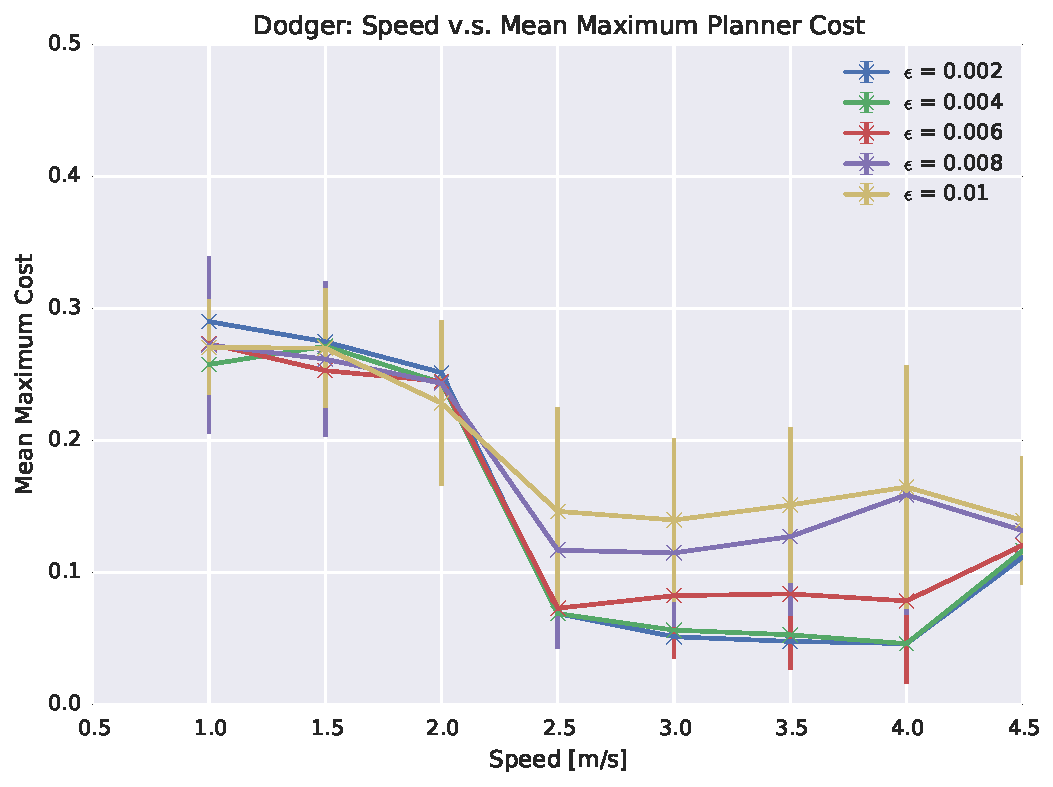
\includegraphics[width=0.49\textwidth]{figs/planner_mean_max_cost_0.pdf}
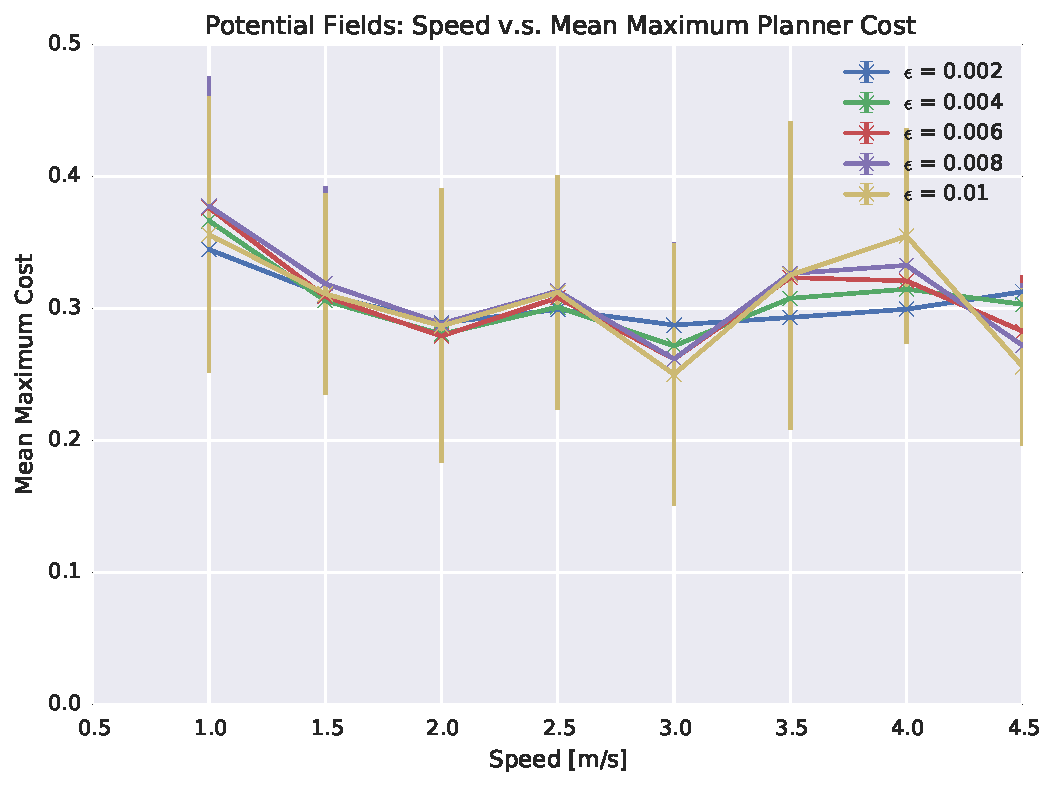
\includegraphics[width=0.49\textwidth]{figs/pf_mean_max_cost_0.pdf}

\end{problock}

      \end{column}

%%%%%%%%%%%%%%%%%%%%%%%%%%%%%%%%%%%%%%%
      \begin{column}{43in}
        \begin{problock}{APPROACH}

{\centerline{
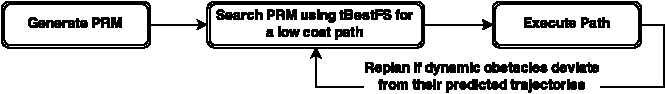
\includegraphics[width=1\columnwidth]{figs/DodgerScheme}
}}

\begin{columns}[t]

\column{0.48\columnwidth}

\textcolor{red}{\textbf{\large{1. Dynamic Obstacle Representation}}}

A dynamic obstacle is represented by five variables:
\begin{itemize}
    \item $I$ is the initial configuration of the obstacle,
    \item $\dot{\zeta}$ is a function, $\dot{\zeta}: \mathbb{R}^+ \rightarrow
\mathbb{R}^2$, representing the velocity of the obstacle
    \item $\epsilon$ is used to define a random variable
        $\rho \sim \mathcal{U}(-\epsilon, \epsilon)$
    \item $\xi$ is the last known configuration of the obstacle used for
        extrapolation
    \item $T$ is the time at which $\xi$ was recorded
\end{itemize}

The cost distribution for a single dynamic obstacle used as a heuristic
for planning is:
\begin{equation*}
    P_a(x, y, t_0, t_m) = \frac{1}{t_m} \cdot \int^{t_m}_{t_0}
    \mathcal{N}(\zeta_a(t), \alpha \cdot (t - t_0)^2 + \beta, x, y) \cdot
    (t_m - t + 1)^{\gamma} \,\mathrm{d}t
    \label{eq:singleprob}
\end{equation*}

Where $[t_0, t_m]$ defines the interval for which the cost distribution is
evaluated on. This serves to represent the likelihood of an obstacle moving
to an $(x, y)$ location between for a time $t$ such that $t_0 \leq t \leq t_m$

\begin{center}
    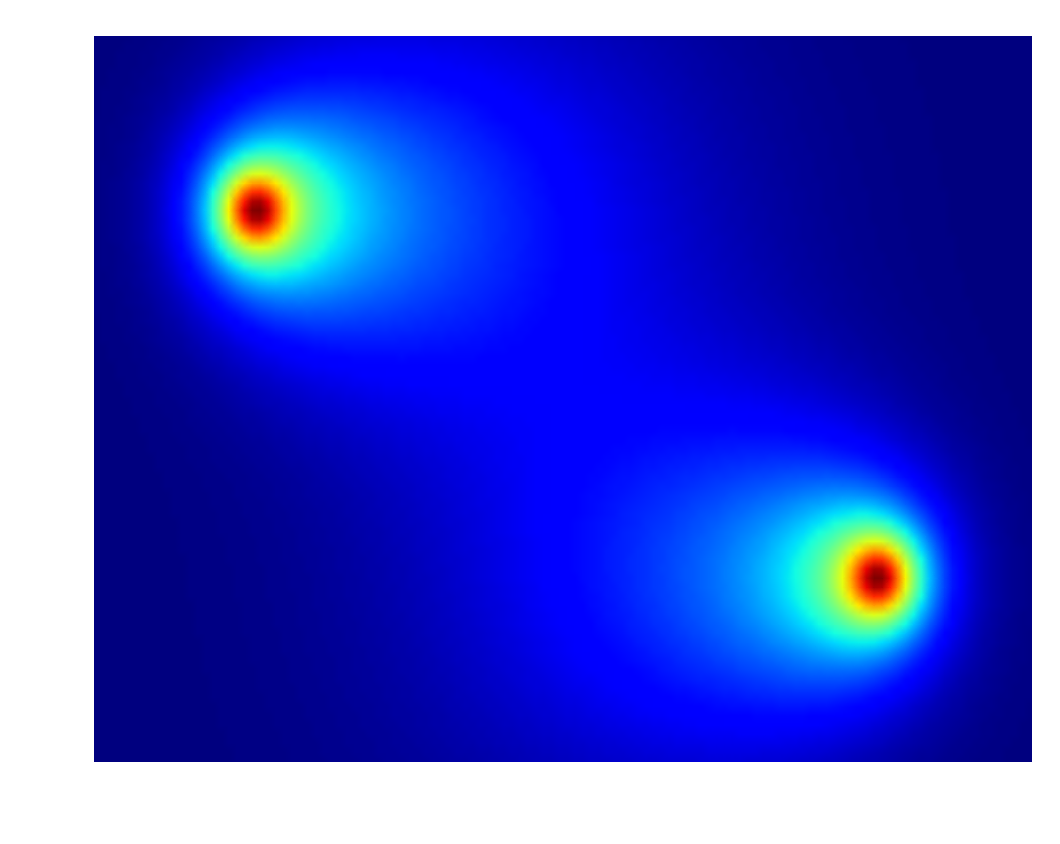
\includegraphics[width=0.49\linewidth]{figs/agent_1}
    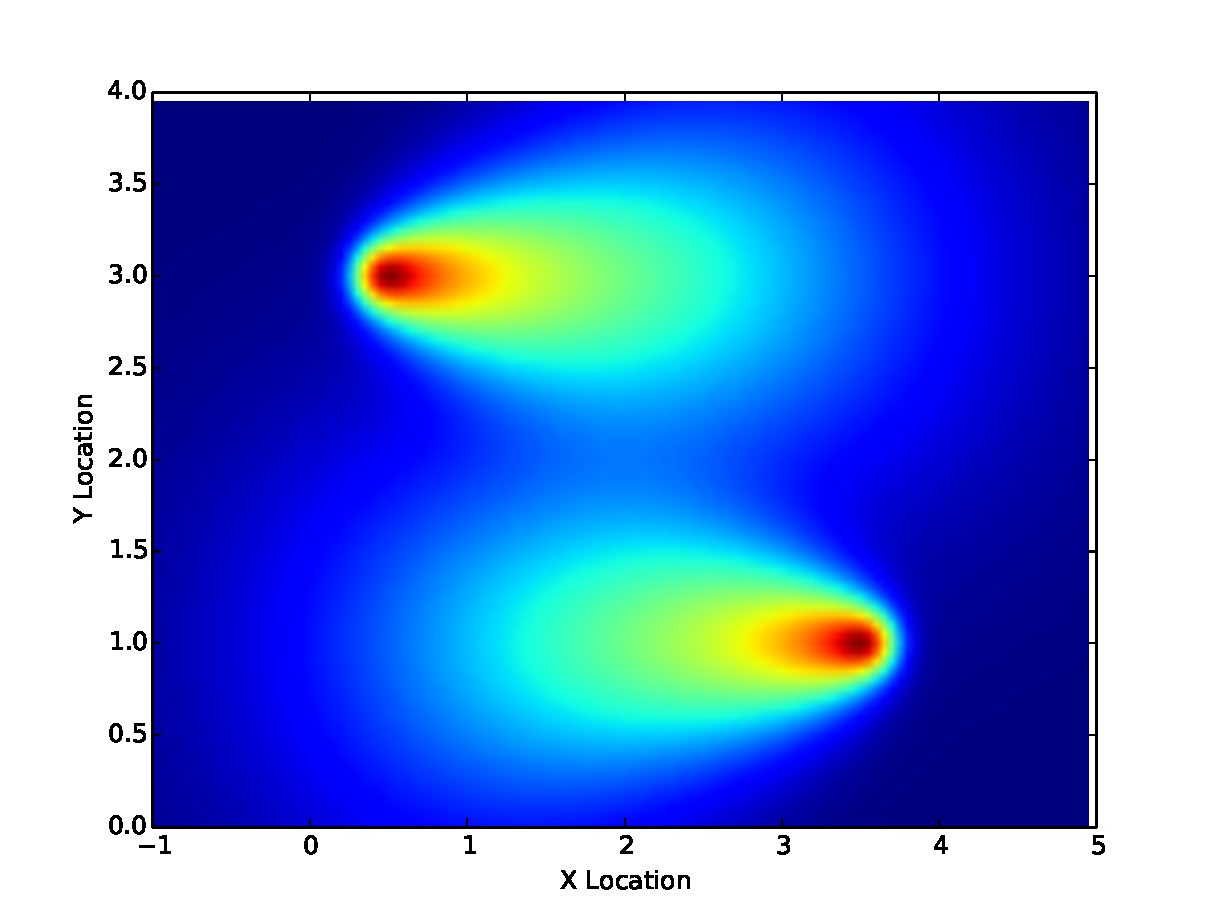
\includegraphics[width=0.49\linewidth]{figs/agent_3} \\
    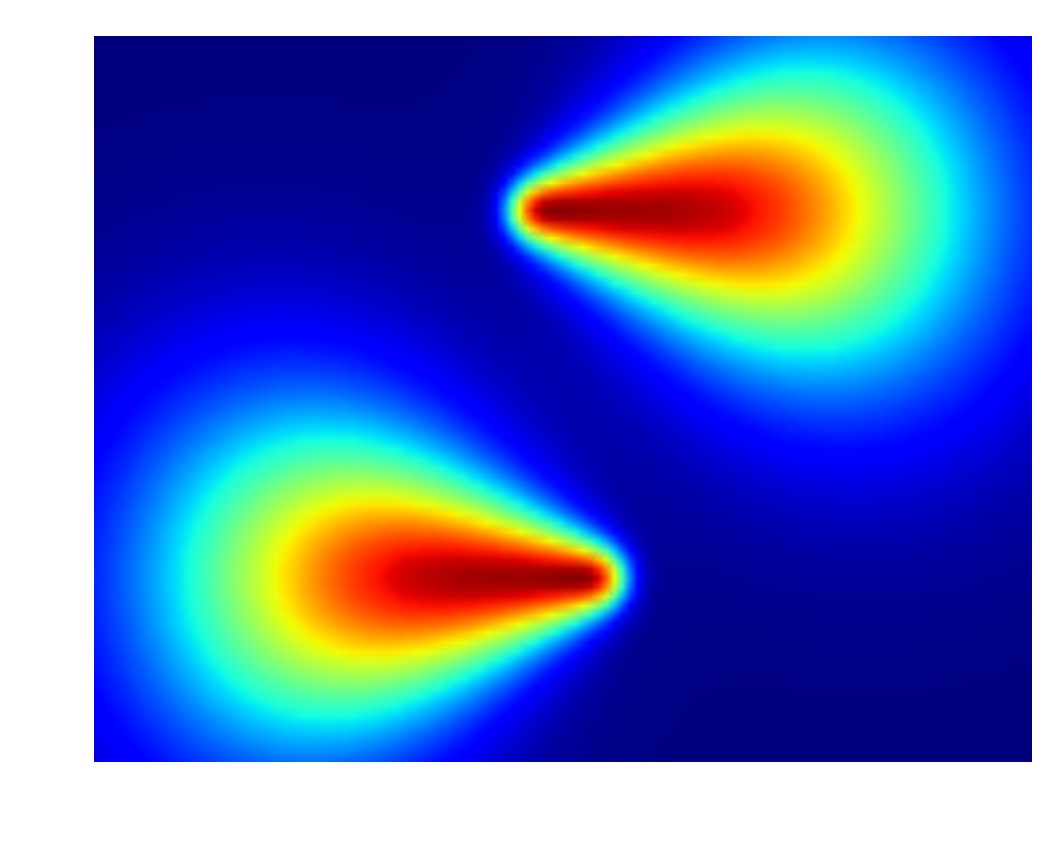
\includegraphics[width=0.49\linewidth]{figs/agent_5}
    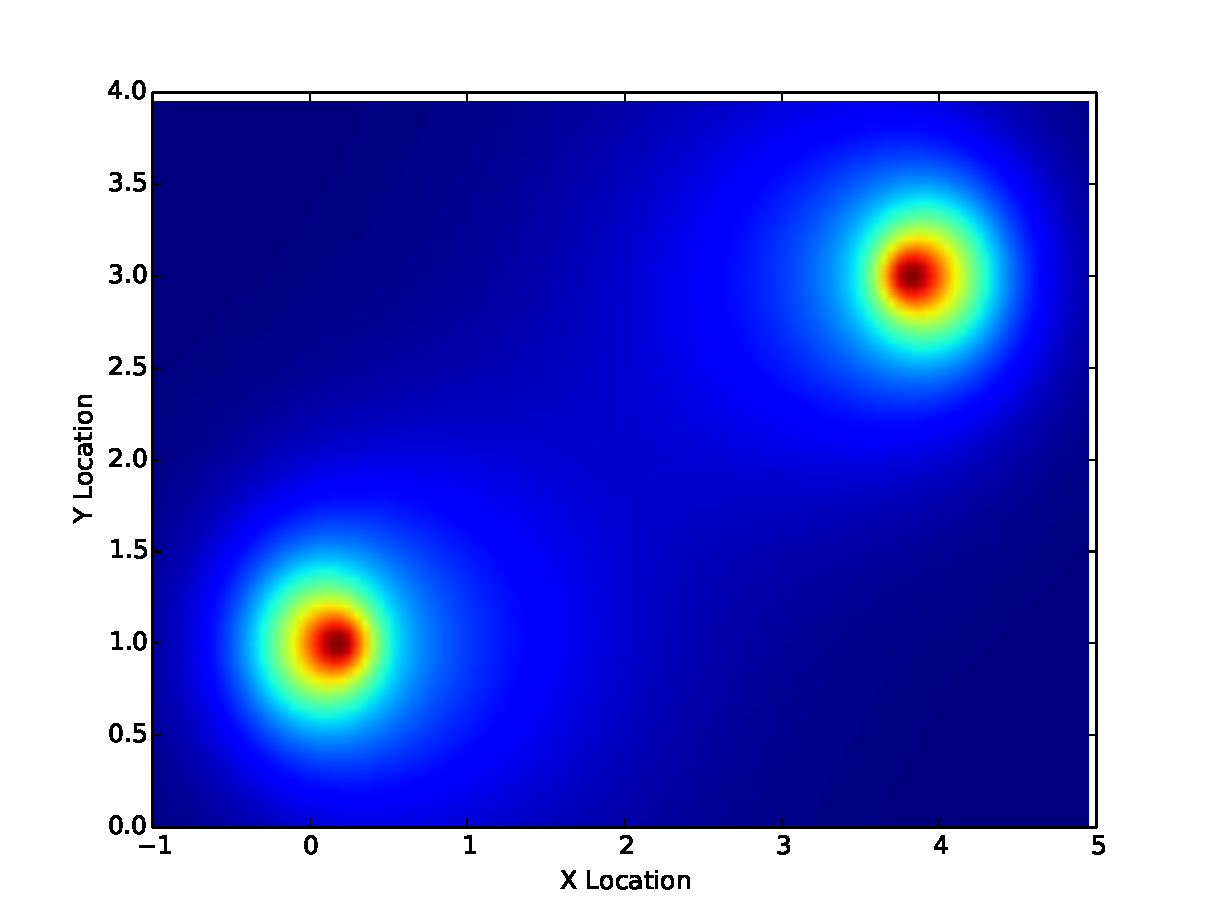
\includegraphics[width=0.49\linewidth]{figs/agent_8}
\end{center}


\textcolor{red}{\textbf{\large{2. Generating the Probabilistic Roadmap (PRM)}}}

\begin{itemize}
\item constructed over the configuration space of the robot
\item used to guide the expansion of the temporal graph search\\[3mm]
\end{itemize}

{\centering{
    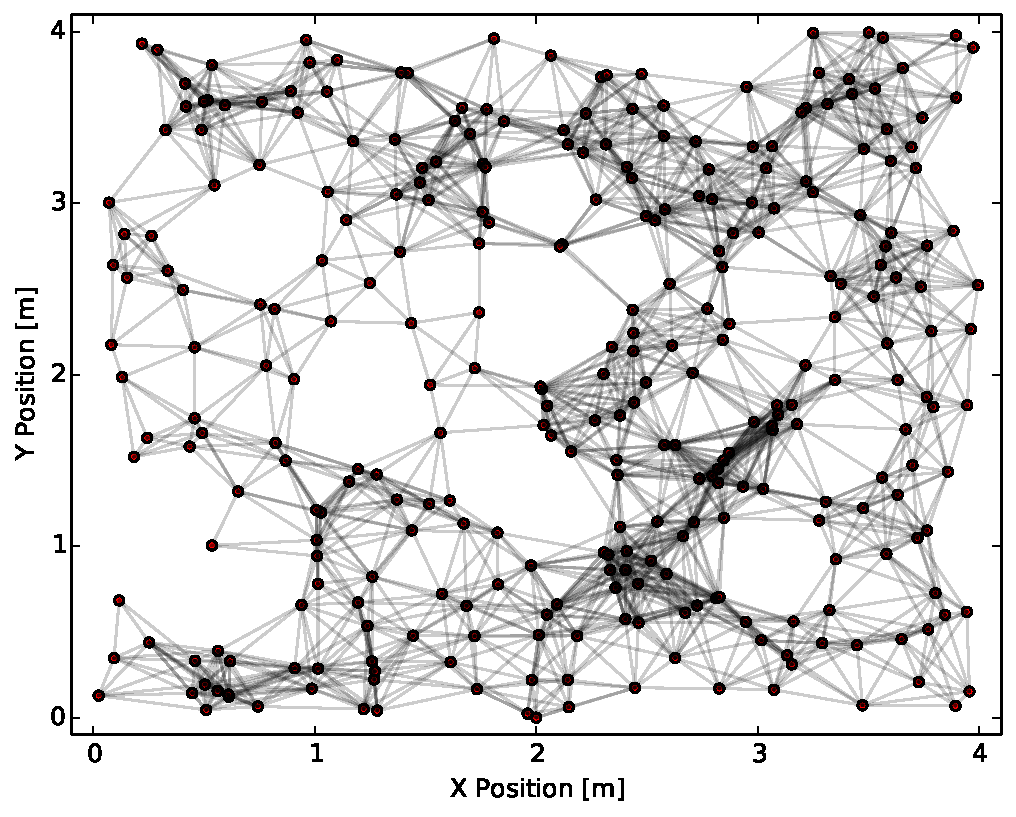
\includegraphics[width=0.8\textwidth]{figs/roadmap}
}}

\vspace*{10mm}

\textcolor{red}{\textbf{\large{2. Heuristic Costs based on the Roadmap Abstraction}}}

\vspace*{8mm}

\begin{itemize}
\item[] \textcolor{mathrgb}{hcost(c)} estimates the difficulty of
  reaching the goal from the roadmap configuration $c \in V_{RM}$:
  defined as the length of the shortest path in the roadmap
  $RM=(V_{RM}, E_{RM})$ from $c$ to the goal

\vspace*{15mm}

\item[]
\textcolor{mathrgb}{$[hcost(v_1), hcost(v_2), \ldots, hcost(v_n)]$}: computed by running Dijkstra's single-source
  shortest-path algorithm over the roadmap $RM = (V, E)$ using the goal vertex  as the source

\end{itemize}

\column{0.48\columnwidth}

\textcolor{red}{\textbf{\large{3. Motion Tree}}}

\vspace*{8mm}

\begin{columns}[T]

\column{0.43\textwidth}

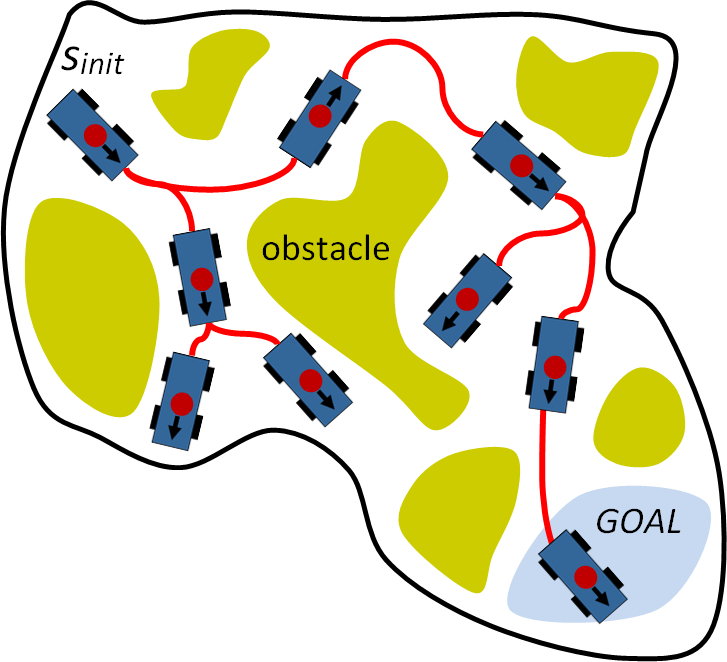
\includegraphics[width=\columnwidth]{figs/figTreeExp}

\column{0.58\textwidth}

\begin{itemize}

\item defined as \textcolor{blue}{$\Symbol{T} =   (V_\Symbol{T},
  E_\Symbol{T})$}

\vspace*{3mm}

\item each vertex \textcolor{blue}{$v \in V_\Symbol{T}$} associated with a
  collision-free state

\vspace*{3mm}

\item each edge \textcolor{blue}{$(v_i, v_j) \in E_\Symbol{T}$} associated with a
  collision free and dynamically feasible trajectory from \textcolor{blue}{$v_i$} to \textcolor{blue}{$v_j$}

\vspace*{3mm}

\item rooted at the initial state

\vspace*{3mm}

\item expanded by adding new vertices and edges

\end{itemize}

\end{columns}


\vspace*{10mm}

\textcolor{red}{\textbf{\large{4. Grouping of Tree Vertices}}}

\vspace*{8mm}

\begin{itemize}
\item roadmap configuration $c \in V_{RM}$ acts as Voronoi site
\item[] containing tree vertices that have $c$ as their closest roadmap
  configuration
\textcolor{blue}{
$$
\mathrm{group}_{\mathcal{T}, c} = \{s : s \in \mathcal{T} \wedge c = \mathrm{NearestCfgRM}(s)\}
$$}
\vspace*{-15mm}
\item motion tree partitioned into different groups
\textcolor{blue}{
$$
\mathrm{groups}_{\mathcal{T}} = \{\mathrm{group}_{\mathcal{T}, c} : c
\in V_{RM} \wedge |\mathrm{group}_{\mathcal{T}, c}| > 0\}
$$}
\end{itemize}

\textcolor{red}{\textbf{\large{5. Selecting a Tree Group for Expansion}}}

\vspace*{8mm}

\begin{itemize}
\item select group with maximum weight
\textcolor{blue}{
$$
\Var{weight}(\Var{group}_{\Symbol{T}, c}) =
\alpha^{\Var{NrSel}(\Var{group}_{\Symbol{T}, c})} / \Var{hcost}(c)
$$}
\vspace*{-14mm}
\item promote expansions from groups with low heuristic costs
\vspace*{3mm}
\item apply selection penalty with \textcolor{blue}{$0 < \alpha < 1$}
  after each selection to avoid overexploration or becoming stuck
\end{itemize}

\vspace*{10mm}

\textcolor{red}{\textbf{\large{6. Expanding the Tree from the Selected Group}}}

\vspace*{8mm}
\begin{itemize}
\item promote expansions along shortest path from $c$ to goal
\begin{itemize}
\item[$\Rightarrow$] select a target configuration $c_\Var{target}$ at random from this path
\end{itemize}
\vspace*{3mm}
\item promote expansions along new directions
\begin{itemize}
\item[$\Rightarrow$] select a target configuration $c_\Var{target}$ at random from the entire configuration space
\end{itemize}
\vspace*{3mm}
\item select vertex $v$ in $\Var{groups}_{\Symbol{T}, c}$ closest to
  $c_\Var{target}$
\item apply controller to generate trajectory from $v$ toward $c_\Var{target}$
\end{itemize}


\end{columns}


        \end{problock}
      \end{column}

 \end{columns}

% Acknowledgment: This work is supported by NSF-IIS-1449505

  \end{frame}
\end{document}
